%%%%%%%%%%%%%%%%%%%%%%%%%%%%%%%%%%%%%%%%%%%%%%%%%%%%%%%%%%%%%%%%%%%%%
%%%
%%% Set these variables appropriately
%%%
\newcommand{\AUTHORS}{Clay Thomas and Gavriel Hirsch}
\newcommand{\TITLE}{You Can't Handle the Lie: Next-Hop Verification in BGP}
\newcommand{\KEYWORDS}{}
\newcommand{\CONFERENCE}{}
\newcommand{\PAGENUMBERS}{yes}       % "yes" or "no"
\newcommand{\TOAPPEAR}{no}
%%%
%%%
%%%%%%%%%%%%%%%%%%%%%%%%%%%%%%%%%%%%%%%%%%%%%%%%%%%%%%%%%%%%%%%%%%%%%

%%%% Setup the document/page
\documentclass[pdftex,twoside,twocolumn,10pt,letterpaper]{article}
\usepackage{ifthen}

\ifthenelse{\equal{\PAGENUMBERS}{yes}}{%
\usepackage[nohead,
            left=1in,right=1in,top=1in,
            footskip=0.5in,bottom=0.75in     % Room for page numbers
            ]{geometry}
}{%
\usepackage[noheadfoot,columnsep=0.2in,
            margin=1in,centering,truedimen]{geometry}
}

\usepackage{wrapfig}
\usepackage{float}
\usepackage{amsmath,amsthm,amssymb,comment}
\usepackage[noend]{algpseudocode}
\usepackage{fancyhdr}
\usepackage[numbers,sort]{natbib}
\usepackage{xspace}
\usepackage{booktabs}
\usepackage{subfigure}
\usepackage[T1]{fontenc}
\usepackage{textcomp}
\usepackage{mathptmx}   % Times + Times-like math symbols
\usepackage{courier}
\usepackage[scaled=0.92]{helvet}
\usepackage[textwidth=1.5in, disable]{todonotes}

\usepackage{color}
\usepackage{graphicx}
\ifthenelse{\isundefined{\wantBW}}{%
  \usepackage[colorlinks]{hyperref}%        % for online version
}{%
  \usepackage[pdfborder={0 0 0}]{hyperref}% % for paper (B&W) version
}
\newcommand{\URL}[1]{\url{#1}}

%%%%% Setup for PDF
\hypersetup{%
pdfauthor = {\AUTHORS},
pdftitle = {\TITLE},
pdfsubject = {\CONFERENCE},
pdfkeywords = {\KEYWORDS},
bookmarksopen = {true}
}

%\setlength{\parindent}{0pt}
%\setlength{\parskip}{0pt}
\renewcommand{\headrulewidth}{0pt}
\newcommand{\Paragraph}[1]{\vspace{-2ex}\paragraph{#1.}}
\setlength{\topmargin}{-.15in}

\ifthenelse{\equal{\PAGENUMBERS}{yes}}{%
  \pagestyle{plain}
}{%
  \pagestyle{empty}
}

\makeatletter\long\def\@makecaption#1#2{
   \vskip 10pt
   \setbox\@tempboxa\hbox{\textsf{#1: #2}}
   \ifdim \wd\@tempboxa >\hsize % IF longer than one line:
       \textsf{#1: #2}\par      % THEN set as ordinary paragraph.
     \else                      % ELSE  center.
       \hbox to\hsize{\hfil\box\@tempboxa\hfil}
   \fi}
\makeatother

\clubpenalty=10000  % Don't allow orphans
\widowpenalty=10000 % Don't allow widows

\title{\textbf{You Can't Handle the Lie: \\Next-Hop Verification in BGP}}
\author{Clay Thomas\\ claytont@cs.princeton.edu
  \and 
  Gavriel Hirsch\\ gbhirsch@cs.princeton.edu }
\date{}

% Compact itemize and enumerate.  Note that they use the same counters and
% symbols as the usual itemize and enumerate environments.
\def\compactify{\itemsep=0pt \topsep=0pt \partopsep=0pt \parsep=0pt}
\let\latexusecounter=\usecounter
\newenvironment{CompactItemize}
  {\def\usecounter{\compactify\latexusecounter}
   \begin{itemize}}
  {\end{itemize}\let\usecounter=\latexusecounter}
\newenvironment{CompactEnumerate}
  {\def\usecounter{\compactify\latexusecounter}
   \begin{enumerate}}
  {\end{enumerate}\let\usecounter=\latexusecounter}

\newcommand{\ignore}[1]{}

\newcommand{\xc}[1]{\mbox{\textit{#1}}}
\newcommand{\la}{\leftarrow}
\newcommand{\ra}{\rightarrow}
\newcommand{\somespace}{\hspace{0.1cm}}

\def\discretionaryslash{\discretionary{/}{}{/}}
\def\discretionarydot{\discretionary{.}{}{.}}
\def\discretionarycolon{\discretionary{:}{}{:}}
{\catcode`\/\active
\catcode`\.\active
\catcode`\:\active
\gdef\URLprepare{\catcode`\/\active\let/\discretionaryslash
                 \catcode`\.\active\let.\discretionarydot
                 \catcode`\:\active\let:\discretionarycolon
        \def~{\char`\~}}}%
\def\URL{\bgroup\URLprepare\realURL}%
\def\realURL#1{\tt #1\egroup}%

\newcommand{\eg}{{\em e.g.}, }
\newcommand{\ie}{{\em i.e.}, }
\newcommand{\etal}{{\em et al.\ }}

\def\check{\stackrel{{\scriptscriptstyle ?}}{=}}

\DeclareMathOperator*{\argmax}{arg\,max}
\DeclareMathOperator*{\val}{val}

\newcommand{\R}{\mathbb{R}}
\newcommand{\N}{\mathbb{N}}
\newcommand{\Z}{\mathbb{Z}}

\newtheorem{definition}{Definition}
\newtheorem{lemma}{Lemma}
\newtheorem{theorem}{Theorem}
\newtheorem{conjecture}{Conjecture}

\begin{document}
\maketitle

\begin{abstract}
  This paper presents a new protocol called \emph{Next-Hop Verification},
  which reduces the set of contexts in which
  autonomous systems are incentivized to lie while participating in BGP.
  The protocol works by sharing information about BGP path announcements
  between different AS's, using the existing structure of the network,
  and checking those path announcements against the true flow of traffic
  in the data plane.
  We discuss the advantages and disadvantages of this new approach,
  and compare its effectiveness to that of previously considered verification
  techniques, focusing on cases where next-hop verification provably eliminates
  the incentives to lie in BGP.
\end{abstract}

\section{Introduction}

  \subsection{Background and Previous Work}
    Routing on the Internet involves many distinct Autonomous Systems (AS's), each
    with its own data sources, destinations, and links; as well as its own
    preferences over how traffic is routed. An AS may prefer that the traffic it
    sends and receives be sent over the shortest path, in order to decrease
    latency; or it may prefer to send its traffic through specific
    other AS's for economic incentives, due to contracts about
    routing costs; or it may prefer to avoid certain other AS's, if it is
    concerned about malicious activity. In the other direction, an AS may also
    prefer to attract or deter traffic from certain other AS's, again for economic
    incentives or perhaps even to spy on certain traffic.

    These AS's typically use the Border Gateway Protocol (BGP) to announce
    routes to neighbors and learn routes from neighbors in the 
    \emph{control plane},
    and to then choose how to actually route traffic in the \emph{data plane}.
    However,
    there is no way for BGP to enforce the requirement that an AS route traffic in a
    way that matches its announcements.
    Thus, due to all of the various (often conflicting)
    preferences that AS's have over how traffic is routed,
    there are incentives to lie in the control plane about what an AS
    will actually do in the data plane, in order to influence how other AS's behave.

    To counteract this, \emph{verification protocols} have been developed which
    run alongside or alter BGP in order to prevent lying.
    Unfortunately, directly verifying the routes a packet takes in the data plane
    requires cryptographic signatures on every packet, as in \cite{DataPlane}.
    This huge overhead makes full data-plane verification impractical.
    Instead, previous work has searched for control plane protocols
    which still manage to prevent or discourage certain types of lies.

    Much work has been done on analyzing BGP control plane
    verification protocols through game-theoretic models.
    In \cite{RoutingGames}, the authors show that in a general set of contexts, a form of
    verification called \emph{path verification}\footnote{
      In the original
      paper they refer to it as route verification.}
    ensures that no AS or group of
    AS's can get strictly preferred routes for its traffic by telling lies.

    However, lying can potentially give other benefits beyond getting better
    routes for your own traffic.
    In \cite{Attraction}, the authors analyze BGP games
    in which agent's utility may depend
    on attracting traffic from other AS's.
    In this scenario, even using path verification does not suffice to
    disincentivize lying.
    They introduce another form of verification
    called \emph{loop verification}, which is simpler but weaker, and describe
    conditions under which path or loop verification do disincentivize lying.
    However, they admit that many of these conditions are unreasonably strong,
    such as requiring that AS's follow an ``all or nothing'' export rule.
    % (for each neighbor, the AS will either announce all paths, or none).

    Another proposal for detecting BGP lies---or more generally BGP faults---is
    NetReview \cite{NetReview}. When using NetReview, AS's record and publish
    all their BGP messages in tamper-evident logs, and other AS's are able to
    audit these logs to check whether there are any faults. However, actually
    detecting the faults requires regularly auditing the entirety of every AS's
    logs which is nontrivial. In addition, NetReview is purely in the control
    plane, so additional work needs to be done if we are concerned that AS's may
    route in the data plane differently than what they announced in the control
    plane. Next-hop verification addresses both of these concerns by being
    relatively simpler, and by incorporating information from the data plane.

  \subsection{Our contributions}
    Given the difficulty of preventing lies in BGP,
    we would at least like to be able to \emph{detect} lies when they are 
    told\footnote{
      For the purposes of our discussion, we assume that AS's always want 
      to avoid being caught lying, so detecting lies is the same as
      disincentivizing those lies.
    }.
    The initial observation of this work is that
    there will always be at least one AS that knows what each
    other AS is truly doing, namely the one that directly receives traffic from
    it in the data plane.
    As a result, if AS's are willing to collaborate then there is
    information that can be used to detect the existence of lies, without
    requiring full data-plane verification. Put another way, we can just monitor
    each AS, rather than every packet.
    Based on this observation, we present a new protocol called
    \emph{next-hop verification}
    and show that it effectively detects lies in certain scenarios.

    As with previous practical verification protocols,
    next-hop verification protocol runs in the control plane.
    However, it also uses
    information sampled from the data plane in order to aid verification.
    Specifically, it requires AS's to keep track of which of its neighbors
    forward traffic towards it for different destinations.
    Given that agents have this information, next-hop verification gives an
    effective way for agents to distribute and answer queries
    about the true data plane paths used by other AS's.
    The distribution of queries uses the existing structure
    of the network and requires no encryption.

    We find that assuming full compliance, next-hop verification allows us to catch lies assuming
    there are is no traffic attraction among preferences.
    In this regard, next-hop verification is similar in effectiveness to 
    path verification.
    In the context where preferences involve traffic attraction,
    we are able to significantly weaken the assumptions which
    \cite{Attraction} needed on the preferences of AS's.
    In this sense, next-hop verification is sometimes more powerful
    than path verification (although there do exist cases where
    path verification will prevent a lie that next-hop verification cannot catch).
    Additionally, we find that next-hop verification is strictly more
    powerful than loop verification, that is, every lying situation detected
    by loop verification will be detected by next-hop verification
    % (though loop verification is still more lightweight).
    In general, we attempt to embark on a similar program to that of
    \cite{Attraction}, experimenting with various settings and seeing
    where next-hop verification leads to good incentive properties.

\section{Model Details}
  \subsection{BGP framework}
    We model the network of AS's as an undirected graph, with a node for each AS
    and an edge between any two AS's that can directly communicate with each other
    without going through a third AS. We assume that the graph is a single
    connected component, so any AS can in theory interact with any other AS.
    As is standard in the literature, we assume there is a unique destination AS
    $d$, because routing to different destination (prefixes) is done
    independently in BGP.

    In the BGP framework, AS's can announce the
    existence or removal of paths to each other.
    Each AS has an import policy that
    determines how it responds to path announcements from neighboring AS's.
    Specifically, the import policy determines whether and how the AS will update
    its route, when it hears new announcements.
    Furthermore, each AS has an export policy that determines whether it will
    announce its current path to a neighbor (or, if the agent is being
    manipulative, it could announce a path different from the one it is actually
    using). These import and export policies are the action space of each agent AS.
    Finally, each AS has some preferences over how the actual traffic in the
    network flows, regarding both what route it gets and how other AS's route through it.
    Each AS will choose a strategy, namely their import and export
    policies, based on these preferences.

    More precisely, there are two types of actions available to each agent:
    installing certain routes in their forwarding table,
    and announcing paths to their neighbors.
    Let $N(i)$ denote the neighbors of AS $i$ in the BGP graph.
    Formally, we could model the import policy of a node $i$ as a function
    $imp_i : Path^{N(i)} \to Path$ from the (possibly empty) collection of
    routes currently announced as available to $i$, to a (possibly empty) path
    to use for forwarding traffic\footnote{
      We actually allow a manipulative, non-BGP compliant agent to have a
      strictly larger set of available actions: the agent may forward down
      multiple routes
    }. We assume that AS's have a utility function $v : Path \to \R$
    which models their preference among the different paths to the destination.
    A non-strategic import policy would simply select the favorite
    path available to the AS at a given point in time.

    The export policy could be modeled as a function
    $exp_i : Path\times N(i) \to Path$ from the current path $i$ uses and a
    given neighbor of $i$ to a path to announce to the neighbor (or the empty
    path if $i$ does not wish to export).
    For a BGP compliant AS, the export policy simply amounts to choosing whether
    to export the path the AS currently uses (that is, we have $exp_i(j, p) = p$ or
    $exp_i(j, p) = []$).
    In realistic settings an AS may prefer not to announce its path to all
    neighbors, the most famous example of this being the Gao-Rexford framework
    \cite{GaoRexford}, in which for example customers will not route traffic
    between two of their providers.
    The export policy may more generally be determined by the traffic attraction
    and repulsion preferences of the AS.
    For a manipulative, non-BGP compliant AS,
    a much richer set of export policies is available:
    the AS can lie arbitrarily, announcing paths that it doesn't use
    or that don't even exist.

    \begin{definition}
      Suppose a BGP network $G$ has reached a stable equilibrium.
      We say that an AS \textbf{m} is \textbf{lying} if the
      it exports a route other than that which it is using.
      We say that an AS is \textbf{honest} if it is not lying.
    \end{definition}

    We assume that the collection of strategies leads the network to converge to a
    stable solution.
    In general contexts, convergence becomes very hard to
    reason about. Because of this complexity and the fact that in practice
    convergence typically does occur (at least for small local subgraphs),
    in this paper we choose to focus on what happens after
    convergence. We show that if the network were to converge to a state that
    depends on lies, then in some scenarios
    we would then be able to catch the lies and shame the liar.
    As a result, it should not be beneficial to lie in a way that leads to that
    state.
    See \cite{RoutingGames, GaoRexford, StablePaths, PolicyPathVector}
    for more formal details about proving different types of convergence
    and what assumptions are necessary.


  \subsection{Verification}
    % CITE SOURCES IN VERIFICATION SECTION
    In this section, we give an overview of some previously considered 
    verification protocols. These will be our comparison points for next-hop
    verification.

    \begin{definition} 
      In a network using \textbf{path verification} it is
      impossible for AS's to announce that they are using paths which were not
      already announced to them.
    \end{definition}

    Some extensions to BGP, such as S-BGP, can enforce path verification
    using cryptography.
    However, it requires additional overhead as well as universal adoption
    \cite{PartialDeploy}, because every route communicated in the control plane
    must be cryptographically signed by every AS along that route.

    \begin{definition}
      In a network using \textbf{loop verification} no AS will
      use an export policy that involves not sending a path to a neighbor
      specifically because that neighbor is already in the path.
      In addition, if an AS $u$ ever sees a path containing $uR$, 
      where $u$ did not actually announce route $R$, it will
      ``raise an alarm'', with the idea that the offender (the first
      node which announced a false path) can be publicly shamed.
    \end{definition}

    Note that if agents' export policies never sent paths to neighbors who are
    already in them, then loop verification could not be done.
    The name loop verification comes from the ``routing loop'' formed by
    announcing a path containing $u$ to AS $u$.

  \subsection{Behavioral assumptions}
    When agents get utility from attracting traffic, stronger verification
    protocols are needed to disincentivize lying.
    In \cite{Attraction}, the authors consider the following classes of
    preferences which depend on more than just an AS's own path.

    \begin{definition}
      An AS $m$ cares about \textbf{volume attraction} if its utility can depend on
      the set of AS's that route through $m$.

      An AS $m$ cares about \textbf{generic attraction} if its utility can depend on
      the set of AS's that route through $m$ AND on the routes these AS's take to get to $m$.
    \end{definition}

    Volume attraction can reflect truly malicious situations such as spying,
    where the manipulative agent wants to view packets for some nefarious
    reason. Issues like this may occasionally have huge consequences for the
    global routing behavior of the internet, for example, the 2010
    China Telecom BGP hijacking could've potentially served this function
    \cite{ChinaHijack}. It could also simply reflect an economic incentive such as
    getting paid for routing more traffic.

    With preferences for generic attraction, an AS $m$ may have incentives to affect
    \emph{how} other agents route through $m$.
    For example, a provider may want a customer to route directly through it
    in order to charge that customer more.

    We briefly consider one assumption on the path preferences of AS's as well:
    \begin{definition}
      An AS $n$ has a \textbf{next hop import policy} if its choice of which path to use
      is a function of only the first AS along the path (i.e. the next-hop).
    \end{definition}

\section{Next-Hop Verification Protocol}
  We now define next-hop verification.
  This protocol is run on a BGP network after convergence has already occurred.
  Nodes communicate along existing links in the network, storing and sending
  next-hop queries. We assume that AS's can ``raise the alarm'', similar to
  \cite{Attraction}, which refers to alerting others that something
  is going wrong with the particular query. For our results section,
  we will assume that when the alarm is raised, the offending agent will be
  caught (for example, via the collaboration of the NANOG mailing list to detect
  the problem, as suggested in \cite{Attraction}), and its lie will be
  disincentivized.

  Each node maintains a queue of queries which it needs to answer.
  A query is denoted $Q_d(a,b)$, representing a node announcing that
  $a$ uses $b$ as its next-hop in its path to destination $d$.

  Whenever $n$ acts, it runs the function {\sc Respond},
  detailed in Figure~\ref{fig:Pseudocode}, on every query
  $Q_d(a,b)$ waiting in its queue, then waits for more queries.

  After $n$ has sent some traffic to $d$, it can start querying about its own
  route. It does this by adding the query $Q_d(a,b)$ to its own queue,
  for every hop $(a,b)$ on $n$'s path to the destination $d$.

  We have sketched an implementation of next-hop verification in Haskell.
  Visit
  \href{https://github.com/ClathomasPrime/Cs561Proj/tree/master/bgp-fact-check/}
  {our repository}\footnote{
    Located at github.com/ClathomasPrime/Cs561Proj/
    under the bgp-fact-check/ directory.
  }
  to check out the code.
  Of particular interest is the file src/FackCheck.hs, which implements the
  above {\sc Respond} in the functions `\texttt{processMessage}' and
  `\texttt{factCheckAnswerQuery}'.

  For a motivating example of next-hop verification, consider the
  network given in Figure~\ref{fig:Nonexistent} (a common example in discussions
  of BGP incentives \cite{RoutingGames, Attraction}).
  Here, $m$ is able to get a preferred path to the destination by falsely
  announcing the path $md$ to node $2$.
  However, nodes $1$ and $d$, which are both one hop away from $2$,
  can tell that this announcement is not legitimate:
  $d$ knows that $m$ does not route directly to $d$,
  and $1$ knows that $m$ routes directly to $1$ instead of $d$.
  If $d$, $1$, and $2$ are all compliantly running next-hop verification,
  $2$ will ask both other nodes the query $Q_d(m,d)$ and both
  will ``raise the alarm''.

  \begin{figure}[h]
    \centering
    \caption{NonexistentPath}\label{fig:Nonexistent}
    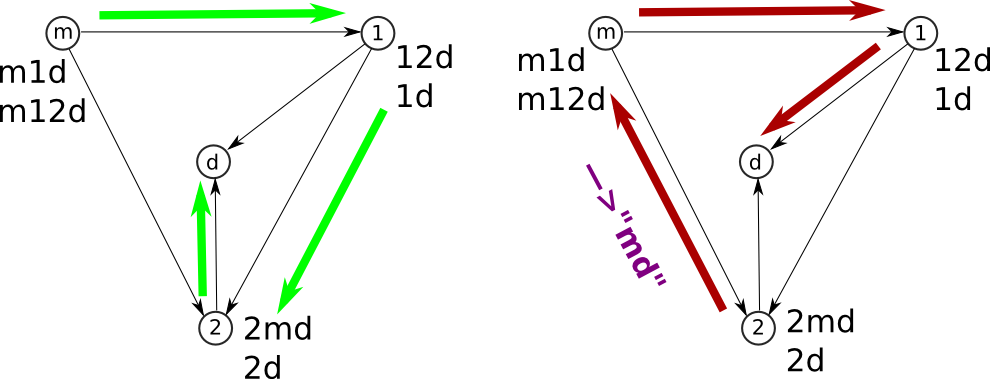
\includegraphics[width=0.5\textwidth]{NonexistentBetter}
  \end{figure}

  \begin{figure}[t]
    % As the document currently is, putting this here was the only way I could
    % get the line numbers to link correctly. Latex is wack
    \centering
    \begin{algorithmic}[1]
      \State Denote the acting AS by $n$
      % \Function{Initialize}{}
      %   \For {each hop $(a,b)$ in $n$'s path to $d$}
      %     \State Add the query $Q_d(a,b)$ to your query queue
      %   \EndFor
      % \EndFunction
      \Function{Respond}{$Q_d(a,b)$}
        \If { $n$ previously responded to $Q_d(a,b)$ }
          \State \Return
        \EndIf
        \If { $n = a$ }
          \If { $n$ does not use $b$ as its next hop for $d$ }
            \State ``raise the alarm'' \label{line:sourceRaise}
          \EndIf
          \State \Return
        \EndIf
        \If { $n = b$ }
          \If { $a$ does not use $n$ as its next hop for $d$ }
            \State``raise the alarm'' \label{line:targetRaise}
          \Else
            \State send the query $Q_d(a,b)$ to all neighbors
              \label{line:falseNegativeForward}
          \EndIf
          % \State send the query $Q_d(a,b)$ to all neighbors
        \Else \ (i.e. $n \neq a,b$)
          \If {$a$ uses $n$ as its next hop for $d$ }
            \State ``raise the alarm'' \label{line:otherRaise}
          \Else
            \State send the query $Q_d(a,b)$ to all neighbors
              \label{line:cluelessForward}
          \EndIf
        \EndIf
      \EndFunction
      % \SetKwFunction{Respond}{Respond}
      % \Function{Main}{}
      %   \For {each query $Q_d(a,b)$ in $queue$}
      %     \State {\sc Respond}($Q_d(a,b)$)
      %   \EndFor
      %   \State clear the $queue$
      % \EndFunction

    \end{algorithmic}
    \caption{Next-hop verification pseudocode}\label{fig:Pseudocode}
  \end{figure}

  We note the following important considerations:
  \begin{itemize}
    \item In the case where $n$ is responding to a query $Q_d(a,n)$, it needs to
      check whether $a$ actually forwards traffic directly to $n$ for
      destination $d$, which must be done in the data plane. Accordingly, each
      AS should keep a flag for each other (neighboring AS) $\times$ (dest AS)
      pair, representing whether the first AS ever directly sends $n$ traffic
      destined for the second $AS$.
      In practice, maintaining the accuracy of this information in the
      face of the dynamic nature of routing would be difficult.
      For example, AS's need to reset the flags after certain lengths of time
      without seeing any traffic.
      However, we leave the details to future work.

    \item We require nodes to actually send traffic before asking next-hop
      queries. This forces the potential manipulator to actually use at least
      some data-plane paths, in the hopes that it will use a false path.
      Intuitively, this will leave evidence of the lie, in the sense that
      certain AS's will know what is actually happening.
      More generally, we assume that enough traffic is sent such that
      all data-plane paths are actually observed, and
      that the absence of traffic means that a given route is not
      being used. This is a strong assumption on the traffic in the network, but
      in very stable networks (and for important destinations) this assumption
      is not too unreasonable.

    \item If a manipulator is lying about the next-hop it is personally using,
      it may intentionally send occasional traffic towards its announced
      next-hop, while sending the bulk of its traffic down the route that it
      genuinely prefers. We take this strategy into consideration, and our
      theorems hold even allowing for this.
      However, it means that if $n=b$ and $a$ forwards traffic directly to $b$,
      then $n$ cannot guarantee that $a$ doesn't forward traffic elsewhere as well.
      Instead $n$ must forward the query on to its neighbors
      in line~\ref{line:falseNegativeForward} of {\sc Respond}.
      Furthermore, it means we cannot rely on line~\ref{line:targetRaise}
      in any of our theorems, because if $a$ is the manipulator
      it may send a small amount of ``fake traffic'' to $b$
      in order to ``cover its tracks''.
  \end{itemize}

  \begin{figure}[h]
    \centering
    \caption{FalsePositive}\label{fig:FalsePositive}
    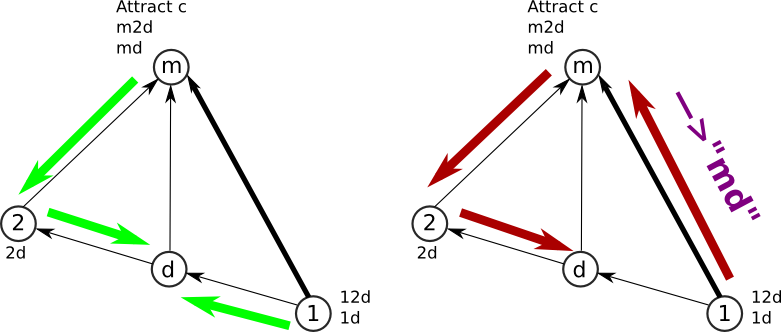
\includegraphics[width=0.5\textwidth]{Inconsistent}
  \end{figure}

  Figure~\ref{fig:FalsePositive}, considered in \cite{Attraction} under the name
  Inconsistent\-Policy, gives another example of next-hop verification,
  and also illustrates the final bullet point above. In this network, $m$ wants
  to carry traffic from $1$, but must lie to $1$ in order for it to choose $m$
  as its next-hop. In order to obscure this lie, $m$ can try to send a small
  amount of its traffic directly to $d$, while still using its favored path
  through $2$ for the bulk of its traffic.
  Running next-hop verification, $1$ will ask the query
  $Q_d(m,d)$ to $d$. Node $d$ will indeed observe a small amount of traffic
  coming from $m$, so it cannot raise the alarm.
  But it will forward the query to node $2$, which will then ``raise the
  alarm''. Note that, assuming $d$ announces the path $md$ to $m$,
  neither path verification nor loop verification can prevent this strategic
  manipulation. So this is a case where next-hop verification gives us a strict
  advantage over existing verification protocols.


\section{Results}

  % The following lemma is the key to our positive results.
  % It explains whey next-hop verification
  % \begin{lemma}
  %   Let $G$ be a BGP instance with the next-hop verification phase.
  %   Suppose all nodes except one manipulator $m$ are next-hop participants.
  %   Assume that $m$ announces to node $v$ a hop $(a,b)$, where in the data plane the
  %   hop $(a,c)$ is used for some $b\ne c$.
  %   (Note that both $b$ and $c$ may be used if $a=m$ and $m$ is ``faking traffic'').
  %   Furthermore, suppose there exists a path from $v$ to $c$ not containing $m$.
  %   Then $m$ with be caught by next-hop verification, and will
  %   receive utility $-\infty$.
  % \end{lemma}
  % \begin{proof}
  %   Let $P$ denote the path from $v$ to $c$ not containing $m$.
  %   Because the activation sequence is fair, every node along the path with
  %   be activated, in the proper order going from $v$ to $c$.
  %   Node $v$ starts with the query $Q(a,b)$, and thus it will eventually travel
  %   to $b$, which will ``raise the alarm'' and give $m$ utility $-\infty$.
  % \end{proof}

  Our first result formalizes the statement ``in a network without
  traffic attraction, next-hop verification will catch all incentivized lies''.
  See figure~\ref{fig:Nonexistent} for a demonstration of this theorem.
  \begin{theorem}
    Let $G$ be a stable outcome of a BGP instance without traffic attraction.
    Suppose there is a single manipulator $m$,
    and all other nodes honestly participate in BGP and in next-hop verification.
    If $m$ lies in order to get a better path to $d$,
    then next-hop verification will catch that lie and shame $m$.
  \end{theorem}
  \begin{proof}
    Assume $m$ lies by announces a hop $(a,b)$ to $v$, where $(a,c)$ is actually in
    a route from $m$ to $d$ for some $c\ne b$.
    (Note that $m$ could send traffic to both $b$ and $c$ if $m=a$.)

    If there exists a path $P$ from $v$ to $c$ that does not contain $m$, then
    because all nodes along $P$ are participating in the next-hop protocol,
    the node $v$ will ask the query $Q_d(a,b)$, which will travel along path $P$
    until $c$ can ``raise the alarm'' in line~\ref{line:otherRaise} of {\sc
    Respond}. So it is sufficient to show that such a path always exists.\\

    Suppose for contradiction that every path from $v$ to $c$ includes $m$.\footnote{This would be a problem because $m$ could drop next-hop queries so that its lie wouldn't be caught}
    We will show that
    this is not compatible with the hypothesis that $m$ got a better path to $d$ by sdlying.
    % (so $m$ can drop the next-hop queries and its lie won't be caught).
    The route from $m$ to $d$ which includes $(a,c)$ must not have loops, so there exists
    a path $P_1$ from $c$ to $d$ not containing $m$.
    If there were a path $P_2$ from $v$ to $d$ which did not contain $m$, then the
    path $P_2P_1$ (the concatenation of $P_2$ and $P_1$)
    is from $v$ to $c$ and would not contain $m$.
    Thus, every route from $v$ to $d$ includes $m$.

    Because all non-$m$ nodes are honest, $m$ must get $v$ to change its route
    to $d$ in order to get a different path by lying to $v$.
    (More technically, there must exists a choice of
    $v$ which picks a different path).
    However, $v$'s route cannot effect $m$'s route to $d$, because
    every route from $v$ to $d$ includes $m$,
    so no route of $v$ nor any consequence of $v$'s route can change the set of
    paths available to $m$.
    This contradicts the assumption that $m$ got a better path by lying.
  \end{proof}

  The next result shows that next-hop verification is at least as
  effective as loop verification in disincentivizing lying in some cases:
  \begin{theorem}
    Let $G$ be a stable outcome of a BGP instance with generic traffic attraction.
    Suppose there is a single manipulator $m$,
    and all other nodes honestly participate in BGP and in next-hop verification.
    Suppose that loop verification, run on the stabilized network,
    would catch $m$'s lie.
    % Suppose that, among all possible strategies of $m$ and executions of BGP,
    % loop verification would catch $m$'s lie at some point during the execution.
    Then $m$ will be caught by next-hop verification on the stabilized network.
  \end{theorem}
  \begin{proof}
    Suppose loop verification would detect a false path $P$ originally announced
    by $m$. Specifically, this means that $P$ contains a subpath $uR$, where $R$ is not
    actually used by $u$, and that some node $q$ adjacent to $u$ installs a route
    containing $P$ (and can announce that path to $u$ to detect the false loop).

    Let $(a,b)$ be the first hop along the path $uR$ which is not used in the
    data plane. When next-hop verification is run, node $q$ will ask the query
    $Q_d(a,b)$. The query will start at $u$, and travel down the path $R$.
    Note that $P$ must be a simple path starting with $m$,
    so $R$ cannot contain $m$.
    Thus, eventually node $a$ will receive the query $Q_d(a,b)$, and will
    ``raise the alarm'' in line~\ref{line:sourceRaise} of {\sc Respond}.
    % As shown above, an AS cannot be incentivized to lie just to get a better
    % path: there must be traffic attraction.
    % Suppose $m$ attracts traffic from some node $v$ by falsely announcing a path
    % $P$ from $m$ to $d$.
    % The manipulator $m$ must announce the path $P$, and paths containing $P$
    % must spread outward through some part of the graph, and $v$ must end up
    % routing through $P$.
    % Consider the tree $T$ of agents who route through $P$ which is minimal among all
    % strategies of $m$ and executions of BGP.
    % That is, $T$ contains the agents which \emph{must} at some point route
    % through $P$ in order for $m$ to attract traffic from $v$.
    % Note that $T\setminus \{m\}$ is connected, because if $T\setminus \{m\}$
    % contained multiple connected components, then $m$ could have not lied to one
    % of the components, yet still attracted traffic from $v$.
    % This contradicts the definition of $T$ as the minimal such tree.

    % % Consider all the AS's that this announcement travels
    % % through to get to $v$. These AS's form a path $Q$ from $m$ to $v$. Note
    % % that, because all non-$m$ nodes are honest, all the nodes in $Q$ must still
    % % have the path containing $P$ installed in the final stable outcome.
    % % ((NOTE: MAYBE Q SHOULD BE A TREE INSTEAD OF A PATH))

    % \todo{this is an absolute unit of a sentence}
    % Now, the only way for loop verification to guarantee to be able to
    % catch $m$ in this lie is if some
    % node $q$ in the tree $T$ is adjacent to a node $u$, such that $P$ contains
    % the path $uR$, where $R$ is a route that $u$ did not announce.
    % Indeed, in this case a route containing $P$ can be announced to $u$ by $q$,
    % and $u$ can raise the alarm for loop verification.

    % Let $(a,b)$ be the first hop along $R$ which is not actually used in the
    % data plane. Note that $m\notin R$.
    % If next-hop verification is used by all non-manipulator nodes, then $v$ will
    % ask the query $Q_d(a,b)$. This query will travel within the tree $T$,
    % through $q$ to $u$, and along $R$ until it gets to $a$.
    % There, agent $a$ will ``raise the alarm'' in line~\ref{line:sourceRaise} of {\sc
    % Respond}, and $m$ will be caught.
  \end{proof}
  Note that an analogue of the above theorem for path
  verification does not hold\footnote{
    For an example, consider figure~\ref{fig:Bowtie}, altered by removing the
    link between nodes $m$ and $l$. The exact same lying strategy is still
    available to $m$ under next-hop verification, but this is not possible if
    path verification is used.
  }.
  In practice, it is reasonable to run loop verification alongside next-hop
  verification, because loop verification is very lightweight\footnote{
    It even makes the above proof more efficient: the query doesn't have to
    travel down the path $R$, it can be immediately answered at $u$.
  }.
  Combined with the extensive discussion in \cite{Attraction} about the 
  capabilities of loop verification,
  the previous result gives us a few different situations in which
  next-hop verification will catch all incentivized lies.
  The rest of this section is dedicated to weakening the requirements
  for those incentive-compatibility properties to hold.

  The following theorem says that next-hop verification will still catch lies
  in networks with volume attraction.
  Indeed, unlike \cite{Attraction} we do not need to make \emph{any} assumptions
  on preferences or behavior (other than assuming \emph{volume} attraction)
  to get this positive result. See figure~\ref{fig:FalsePositive} for an example
  of this theorem.
  \begin{theorem}
    Let $G$ be a stable outcome of a BGP instance with traffic volume attraction.
    Suppose there is a single manipulator $m$,
    and all other nodes honestly participate in BGP and in next-hop verification.
    If $m$ lies in order to attract traffic from some node $u$,
    then next-hop verification will catch that lie and shame $m$.
  \end{theorem}
  \begin{proof}
    % As shown before, $m$ cannot get a better path. We show further
    % that $m$ cannot attract more traffic (in volume).
    % Let $v$ denote a node that $m$ lied to that affected $u$'s route,
    % and suppose $v$ is told
    % Because the lie told to $v$ affects the path chosen by $u$,
    % there must exist a path $R$ from $u$ to $v$ not including $m$
    % (if not, the lie could only affect $u$ by going back through $m$,
    % in which case $v$ did not have any effect).

    Suppose $m$ did manage to attract more traffic from a victim $u$ by
    announcing a false path $L$.
    Because $u$ routes through $m$ and no node other than $m$ lied,
    $u$ must install a route containing $L$.
    (More technically, there must exists a choice of
    $u$ which installs routes $L$, or else $m$ did not attract traffic by lying.)
    Assume that $L$ contains a hop $(a,b)$, yet data plane hop
    $(a,c)$ is actually used for $c\ne b$.

    Let $P$ denotes the path $u$ would have otherwise taken to $d$.
    Note that by our assumption and the definition of volume attraction, $m\notin P$.
    Now, in the data plane $m$ uses some route $Q$ containing hop $(a,c)$.
    Let $R$ be the subpath of $Q$ which routes from $c$ to $d$,
    and note that $m\notin R$ because $Q$ is a simple path.
    Thus, by eliminating any possible loops from $PR^\top$,
    the concatenation of $P$ with $R^\top$ (the reverse of path $R$),
    we get a simple path from $u$ to $c$ which does not include $m$.
    Because all non-$m$ nodes are actively and honestly running next-hop,
    the query $Q_d(a,b)$ will travel from $u$ to $c$ and $c$ will
    ``raise the alarm'' in line~\ref{line:otherRaise} of {\sc Respond}.
  \end{proof}

  However, we are not able to extend this result to generic attraction.
  Indeed, consider the example given by Figure~\ref{fig:Bowtie},
  taken directly from \cite{Attraction}.
  In this network, the manipulator $m$ wants nodes $n$ and $c$
  to use $m$ as their next hop for destination $d$,
  for example, because of economic considerations.
  The AS's who know what $m$ is doing in the data plane
  are separated from the AS's $m$ is lying to.
  Those victim agents cannot communicate with $d$ and $l$ without
  going through $m$, which can just throw their next-hop queries away
  to avoid being caught.
  \begin{figure}[h]
    \centering
    \caption{Bowtie}\label{fig:Bowtie}
    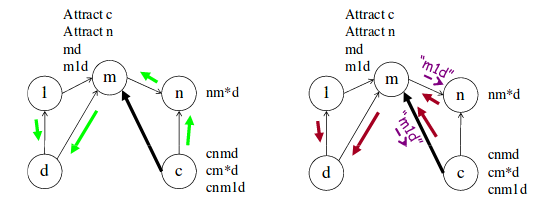
\includegraphics[width=0.5\textwidth]{Bowtie}
  \end{figure}

  We note also that next-hop verification is able to catch the manipulator in
  many of the other examples from \cite{Attraction} (indeed, next-hop verification
  works for all examples except Bowtie and DisputedPath).
  This may hint at many more theorems that we were unable to prove for this
  project. For example, we make the following conjecture:
  \begin{conjecture}
    Let $G$ be a stable outcome of a BGP instance with generic traffic attraction.
    Suppose there is a single manipulator $m$,
    and all other nodes honestly participate in BGP and in next-hop verification.
    Furthermore, assume all nodes use next-hop import policy in ranking their paths.
    If $m$ lies in order to attract traffic from some node $u$,
    then next-hop verification will catch that lie and shame $m$.
  \end{conjecture}
  Intuitively, this should eliminate examples like Bowtie, where the victim node
  $c$ was tricked into routing directly through $m$ because its import policy was not
  next-hop.
  % ((NOTE: the right assumption in the above might be some sort of ``next-hop
  % attraction'', which sounds similar to AT4 from Goldberg. However, discussing AT4 
  % takes us way too far down the Gao-Rexford rabbit hole)).


\section{Possible future directions}

  We showed in the previous section that next-hop verification has the potential
  to provide some major benefits for catching lies in BGP, and thus reducing or
  even eliminating ASs' incentives to do so. However, there is still some future
  work that should be done before it is used in practice.

  One important question is how effective the protocol can be in partial
  deployment or participation. In our theorems we assumed that there was only
  one malicious AS and that all others actively participated fully in helping to
  catch lies. However in practice, it may be the case that some AS's have not
  deployed the necessary software and/or hardware for participation. It may also
  be the case that some AS's choose not to participate or to only share a
  limited subset of the information they have, even if they are not themselves
  malicious, lying agents.
  Partial deployment and participation would still be somewhat valuable though;
  certainly lies can still be detected if we get lucky and all the right agents
  participate. However, a formal analysis with strong theorems is probably
  difficult in the face of such partial deployment.

  A related and interesting line of investigation would be into the
  actual incentives of mutual participation in next-hop verification.
  There are examples where a non-lying agent actually gets a preferred outcome
  through the lies of a manipulator, AND that agent's participation is needed to
  catch the manipulator with next-hop verification.
  In practice, perhaps this ``fact-checking'' could be written into
  customer-provider contract agreements,
  e.g. providers helping customers keep track of \emph{other} providers.
  In the setting of Gao-Rexford networks \cite{GaoRexford}, it may be possible
  to prove strong results, such as participation in next-hop with your customers
  never being harmful.

  Perhaps the biggest practical problem with our protocol
  is the way it ``floods'' the AS graph with next-hop queries.
  In practice, the very minimum that would need to be added is a
  ``time to live'' field on the next-hop queries,
  which would prevent them from exploding over the entire AS graph.

  The clear alternative to this ``query flooding'' is to simply encrypt the
  query and send it to the AS's who can answer it, in the same way that
  one would send normal traffic.
  The burden of such encryption would not be very heavy, and the
  resulting protocol would be more practical for checking on hops which
  are far away from you in the AS graph.
  However, an important aspect of our protocol is the ability for AS's that
  are involved in the actual route but not the fake route to raise the alarm.
  In addition, it seems ideal for a fact-checking protocol to make use of local
  information, like path verification (with local cryptographic signatures)
  or loop verification.
  Indeed, in examples like Figure~\ref{fig:Nonexistent}, the next-hop query
  needs to travel only one hop before being answered.
  In today's very dense AS graph, that may often be the case,
  and with more refined knowledge of the nearby structure of the graph,
  an AS may be able to intelligently route its next-hop queries to get efficient
  answers. We view our protocol, and the theorems surrounding it, as a step
  towards a more refined next-hop verification capable of meeting these
  criteria.


\section{Conclusion}
  In this paper we have proposed the design of Next-Hop Verification, a protocol
  for catching BGP lies by using information from the control plane along with
  minimal information sampled from the data plane,
  and by having the AS's collaborate with each
  other to detect these lies. We also analyzed the theoretical capabilities of the
  protocol, and showed that in many circumstances it is capable of catching lies
  that loop verification and path verification cannot catch. We believe that
  Next-Hop Verification's approach of sharing informationand cross-checking with
  the data plane is a valuable one, and that the protocol is a valuable step in
  working toward more secure control-plane communication.


\bibliography{proj}{}
\bibliographystyle{alpha}

\clearpage

\end{document}

